%% JAAMAS submission (Springer Nature LaTeX template, December 2024 version).
%% Generated by _build_jaamas_tex.py from ../paper/main.tex; edit the source, not this file.
%% Compile: pdflatex -> bibtex -> pdflatex -> pdflatex
\documentclass[pdflatex,sn-mathphys-num]{sn-jnl}

\usepackage{graphicx}%
\usepackage{amsmath,amssymb,amsfonts}%
\usepackage{xcolor}%
\usepackage{textcomp}%
\usepackage{booktabs}%
\hypersetup{bookmarksdepth=2}% run-in \paragraph heads under a \section are not bookmark levels
\renewcommand{\topfraction}{0.85}%
\renewcommand{\bottomfraction}{0.6}%
\renewcommand{\textfraction}{0.12}%
\renewcommand{\floatpagefraction}{0.75}%
\theoremstyle{thmstyleone}%
\newtheorem{proposition}{Proposition}% acmart predefines it; sn-jnl leaves theorem setup to the author

\raggedbottom

\begin{document}

\title[Decision-Time Bounds on Checking LLM Agents]{Looking in the Right Place, at the Right Time: Decision-Time Bounds on Checking LLM Agents}

\author*[1]{\fnm{Haoyang} \sur{Li}}\email{kngonthetrack@gmail.com}

\affil*[1]{\orgname{Irvine Valley College}, \orgaddress{\city{Irvine}, \state{CA}, \country{USA}}}

\abstract{An overseer of agents built on large language models (LLMs) sees only part of a run and must act before failure becomes irreversible. We model a check as a read of the trajectory so far, costing one unit of a fixed budget, and show that when flagged agents are removed for good, a schedule prevents failure exactly when one of its checks falls inside the run's prevention window: from the first round at which the detector can identify the faulty agents to the last at which removing them still helps. On a multi-agent benchmark where a committed minority captures a group's beliefs (60 settings, 50 seeds, every schedule of up to three checks), every window is an interval and the rule predicts all but 8 of 642{,}460 multi-check outcomes. Within a setting windows open in the same round, so one check there attains the clairvoyant bound and more checks add nothing, while evenly spaced checks that start later have prevention rates 0.39 lower. One round of reading delay halves the benchmark detector's median clairvoyant bound, because it needs two messages per agent, and costs nothing for detectors that need only one. Settings no schedule helps are captured in the first rounds or rarely. On a rule-shift stream with random onset, early schedules miss every shift at budgets up to four. On 130 LLM-agent panels, the monitor that ranks agents best on completed transcripts needs history the deadline lacks, and its ranking accuracy falls from 0.95 to 0.56.}

\keywords{agent oversight, monitoring, attention budget, decision-time evaluation, multi-agent systems, large language model agents}

\maketitle


\section{Introduction}

Agents built on large language models (LLMs) now run long, multi-step tasks, and someone has to watch them. Watching every step is too expensive, so oversight in practice means sampling: an overseer, or an automated monitor acting for one, inspects a few points of a run and intervenes if something looks wrong. In this paper the intervention is automatic: a check that flags an agent removes it from the run. A check made early sees only the part of the trajectory that exists so far, which may not yet contain the evidence of a fault. A check made late may find the fault after it can no longer be undone.

Prior work approaches this problem from two directions. Confirmation-scheduling models decide when a user should verify an agent's progress, assuming that a check detects any error present and that errors can be repaired by redoing a step~\cite{zhou2026whenshouldcheck}. Research on artificial intelligence (AI) control measures oversight under a limited auditing budget, but scores monitors on completed transcripts and treats the overseer as acting without delay~\cite{greenblatt2024aicontrol}. Neither assumption holds in the setting we study. A content monitor that reaches an area under the receiver operating characteristic curve (AUC) of 0.91 on finished multi-agent transcripts identifies none of the responsible agents at the last round where removing them would still prevent failure, once the overseer reads one round behind (Section~\ref{sec:hindsight}).

We make this precise with a small model. A check at time $t$ reads only the causal prefix of the run, uses one unit of an attention budget $B$, and changes the outcome only if it comes early enough. Under conditions stated in Section~\ref{sec:model}, each run has a \textbf{prevention window}, an interval of rounds that opens when the detector can first identify the faulty agents and closes when removing them stops helping, and a schedule prevents the failure exactly when one of its checks lands in the window. The window explains when budget matters, what latency costs, and where checking cannot help. We test it on a benchmark where every schedule can be enumerated and use it to answer five questions, in this order:

\begin{enumerate}
  \item What decides whether a checking schedule prevents a fault, and when does a larger budget help? (Section~\ref{sec:s1})
  \item What does one round of overseer latency cost? (Section~\ref{sec:latency})
  \item Where does no schedule help, and why? (Section~\ref{sec:ceiling})
  \item Does an early schedule transfer to faults whose onset is random? (Section~\ref{sec:s2})
  \item Do monitors that look accurate on completed transcripts detect faults in time? (Section~\ref{sec:hindsight})
\end{enumerate}

One check inside the window is all a budget buys when the windows of different runs overlap, and extra checks pay only for windows that move, as they do when onset is random or an adversary avoids known checks. Latency costs what the detector's need for history costs. Settings that no schedule helps are those captured before the first allowed check or captured too rarely to matter. And accuracy on completed transcripts overstates detection at the deadline, because the most accurate transcript monitors rely on history that does not yet exist when a check could still help.

\paragraph{Contributions}
\begin{enumerate}
  \item A model of oversight checks under a budget and a deadline, and a window rule (Proposition~\ref{prop:window}) that reduces any schedule's outcome to whether it hits the run's prevention window. On the capture benchmark, windows are intervals in every captured run and the rule predicts all but 8 of 642{,}460 multi-check outcomes (Sections~\ref{sec:model} and~\ref{sec:s1}).
  \item Evidence on when budget matters. With faults that start at once, one check at the window's first round attains the clairvoyant bound over all 469 schedules, and a second or third check adds nothing; evenly spaced checks starting at round 5 have prevention rates 0.39 lower. A schedule-aware adversary and random onset move the window, and then the fixed early check fails (Sections~\ref{sec:s1} and~\ref{sec:s2}).
  \item Evidence that latency costs what the detector's history requirement costs: one round of reading delay halves the median clairvoyant bound for a detector that needs two messages per agent and leaves perfect and single-message detectors unchanged; the same mechanism explains the timing failures of monitors on LLM panels (Sections~\ref{sec:latency} and~\ref{sec:hindsight}).
  \item Evidence that hindsight evaluation overstates timely detection: across thirteen monitors and 130 panels, the best monitor on transcripts falls from 0.95 to 0.56 AUC at the deadline, and the best recall at the deadline at a 6.25\% false-positive rate is 0.36 (Section~\ref{sec:hindsight}).
\end{enumerate}

\section{Related Work}
\label{sec:rw}

\paragraph{When to check an agent}
Zhou et al.\ cast the placement of user confirmations in multi-step agentic tasks as a scheduling problem that trades checking cost against the cost of redoing work~\cite{zhou2026whenshouldcheck}. Their model assumes that a check detects any error present and that errors stay repairable. We relax both: detection depends on what the prefix contains, and failure becomes irreversible. The AI-control line studies protocols in which a trusted monitor routes suspicious actions to a limited human audit budget~\cite{greenblatt2024aicontrol}, extended to mid-trajectory resampling~\cite{bhatt2025ctrlz}, and evaluates them by end-of-run safety. Turan sets escalation rates for a reviewer whose capacity declines with use~\cite{turan2026capacity}, and Zhang et al.\ argue that failure predictors should be judged by the value of the interventions they enable~\cite{zhang2026calibration}. We share this decision-time view and add the placement of checks relative to fault dynamics.

\paragraph{Inspection schedules, change detection, and strategic auditing}
Choosing when to inspect a system whose failure is revealed only by inspection is a classical problem in reliability: Barlow, Hunter, and Proschan derived optimal checking schedules for a known failure-time distribution~\cite{barlow1963checking}, and Sengupta treated failures whose symptoms appear only after a delay~\cite{sengupta1980delayed}, which is the situation of a detector that needs history before it can flag an agent. Quickest change detection asks when to declare a change~\cite{page1954,wald1945,shiryaev1963,veeravalli2014qcd}; its data-efficient form also decides at each step whether to pay for an observation~\cite{banerjee2012dequickest}. Our window rule is a special case of this inspection view for one-shot removal, and the onset-dependence we report in Section~\ref{sec:s2} is what these models predict. What we add is the measurement for agent oversight: windows of multi-agent capture runs, how a detector's history requirement and the overseer's latency move them, and how monitors evaluated on completed transcripts misjudge them. When the monitored party anticipates inspections, deterministic schedules can be evaded and randomized ones are needed, as in Stackelberg security games~\cite{paruchuri2008playing} and audit games~\cite{blocki2015auditgames}; Section~\ref{sec:s1} tests one such adversary.

\paragraph{Committed minorities and network interventions}
A committed minority that never changes its opinion can flip a population once it exceeds a tipping point, in models~\cite{xie2011committed} and in experiments with people~\cite{centola2018tipping}. Removing agents from a network to stop a spread is the problem of network immunization, where targeting hubs is most effective~\cite{pastorsatorras2002immunization}, and the timing of countermeasures matters for limiting misinformation~\cite{budak2011limiting}. Our checks remove agents, but only those a detector flags from what they have said so far, and only at budgeted times.

\paragraph{Monitoring agents and evaluating monitors}
Interfaces for watching agents include trace explorers and steering consoles~\cite{epperson2025agdebugger,xie2024waitgpt,agentgui2026}, approval-gated orchestration~\cite{magneticui2025}, and visual analytics over agent logs~\cite{agentlens2025}. Monitors are usually evaluated on finished trajectories: SHADE-Arena reports AUC over completed transcripts~\cite{shadearena2025}, and weak-to-strong monitoring reports true-positive rates at fixed false-positive rates on finished runs~\cite{weaktostrong2025}. Anomaly detectors for multi-agent systems work over execution graphs~\cite{sentinelagent2025,gammaf2026} or localize the first faulty step of a completed trajectory~\cite{trajad2026}, and proactive monitors predict unsafe states before they occur~\cite{probguard2026}. Our timely recall plays the role that timeliness-aware scores play in streaming anomaly benchmarks~\cite{nab2015}. That human operators sample instruments rather than watch them continuously is classical~\cite{senders1964,sheridan1992}, as is the finding that passive monitoring fails~\cite{parasuraman1997} and that the timing of an interruption matters as much as its frequency~\cite{iqbal2007disruption}.

\section{Model and Experimental Setup}
\label{sec:model}

\subsection{Checks, budgets, and windows}
A run unfolds over rounds $t = 1, \dots, T$. A \textbf{check} at round $t$ reads only the causal prefix, the messages available at $t$, never the completed transcript; it uses one unit of a budget of $B$ checks per run; and every agent it flags is removed for the rest of the run. A placement policy maps $(B, T)$, and possibly cheap online signals, to check rounds. We report three outcomes: the \textbf{prevention rate}, the share of runs that fail without checks minus the share that fail with them, an absolute difference; the \textbf{timely-catch rate}, the share of runs in which a check removes a faulty agent no later than the failure round; and the \textbf{false-intervention rate}, the share of runs without a fault in which a check removes anyone.

For a run $\omega$, let $W(\omega)$ be the set of rounds $r$ at which a single check would prevent the failure. Four conditions make $W$ an interval and decide every schedule: (A1) a check that flags no one leaves the run unchanged; (A2) a check flags either no one or exactly the faulty agents, who are then removed for good; (A3) once a check can identify the faulty agents, any later check can too; (A4) if removing them at round $r$ prevents the failure, removing them at any earlier identifying round does too. Let $a(\omega)$ be the first identifying round and $b(\omega)$ the last round at which a single check prevents the failure.

\begin{proposition}[Window rule]
\label{prop:window}
Under (A1)--(A4), $W(\omega) = [a(\omega), b(\omega)]$, possibly empty, and a schedule $S$ prevents the failure of $\omega$ if and only if $S \cap W(\omega) \neq \emptyset$.
\end{proposition}

\begin{proof}
By (A1) the run until the first check that flags anyone coincides with the unchecked run, so by (A3) that check is $r_1 = \min (S \cap [a, T])$. By (A2) it removes every faulty agent, later checks flag no one, and by (A1) the outcome equals that of a single check at $r_1$. That check prevents the failure if and only if $r_1 \le b$, using (A4), and since $r_1 \ge a$ this holds if and only if $S$ meets $[a, b]$. Taking $S$ to be a single round gives $W = [a, b]$.
\end{proof}

Two consequences organize the results. First, for any single run one check at $a(\omega)$ does what any schedule can, so the clairvoyant bound, the best schedule chosen separately for each run, does not depend on the budget. For a fixed schedule applied across runs, the prevention rate is the probability that $S$ meets the window: if one round lies in every nonempty window, one check there reaches the bound, and further checks are worth only as much as the windows of different runs fail to overlap. Second, reading delay acts only on $a$. A check whose detector needs $k$ messages from an agent, made with $\ell$ rounds of delay, can identify it no earlier than round $k + \ell$, while $b$ depends on when removal acts, which delay does not change. Delay therefore costs nothing when $k + \ell$ does not exceed the first allowed check round, and otherwise removes the rounds before $k + \ell$ from every window.

The benchmark detector can flag an honest agent, which breaks (A2); Section~\ref{sec:s1} measures how much this matters.

\subsection{Latency}
Within a round, agents send messages, a scheduled check reads what has been sent, flagged agents are removed, beliefs update, and failure is evaluated. Deciding ``at round $t$'' can mean reading rounds $1..t$ (\textbf{zero latency}: the overseer acts within the round) or rounds $1..t{-}1$ (\textbf{one round of latency}: the overseer reads one round behind and acts at the same point).

\subsection{Substrates}
\textbf{Belief capture.} $N{=}32$ agents exchange messages for $T{=}15$ rounds on a communication graph. Each honest agent holds a log-odds belief about a binary state, initialized from a private signal of strength $e$: a fraction $e$ of honest agents receive the true signal, with log-likelihood ratio $\pm\log(e/(1-e))$. Every round each agent announces a claim (the sign of its belief), a confidence $0.5 + 0.5\tanh(|b|/2.5)$ clipped to $[0.51, 0.99]$, and its private signal as cited evidence. A committed minority, placed on the highest-degree nodes, announces the false claim at confidence 0.99 with fabricated supporting evidence from round 1 and never updates. Honest agents update their belief as a weighted average of the previous belief and the private signal (anchor 0.12) plus a social term, the confidence- and support-weighted mean claim of neighbors' messages from the last three rounds with removed senders excluded (weight 2.1), clipped at $\pm 6$. \textbf{Capture} occurs when at least 80\% of honest agents hold the false claim. We vary the number of committed agents (1, 2, 3, 4, 6), $e$ (0.58, 0.66, 0.74), and the graph (hub, random, small-world, clustered), giving 60 settings, which we call \textbf{cells}, each run with 50 seeds, plus 12 cells with no committed agents for measuring false interventions. A check runs the benchmark's content-anomaly score, the \textbf{benchmark detector} described in Section~\ref{sec:hindsight}, on the visible prefix and removes every agent scoring at least 0.5. Policies place $B \in \{1, 2, 3\}$ checks: uniform ($\{8\}$, $\{5, 10\}$, $\{4, 8, 11\}$), random, front-loaded, back-loaded, audit-early (rounds 2, 4, 8, as in audit-budget practice~\cite{greenblatt2024aicontrol}), suspicion-triggered (a check when the round's mean confidence rises above a threshold calibrated on fault-free runs), and an \textbf{onset-informed reference} that checks in the rounds up to and including the capture round. The sweep comprises 72{,}000 trials: 63{,}000 policy runs on the committed cells, 5{,}400 on the fault-free cells, and 3{,}600 unchecked baselines.

\textbf{Rule shift.} A reasoner answers a stream of 160 inputs whose generating rule switches from a source to a target rule at a step drawn uniformly from $[40, 120]$, unknown to the monitor. A check runs a fixed battery of eight probes and updates a posterior over candidate rules. We vary separability (the fraction of inputs on which the two rules disagree) over ten cells ranging from 0 to 0.71 and whether the candidate set contains the target rule, with $B \in \{1, 2, 4, 8, 16\}$ and 24 seeds (14{,}400 trials).

\textbf{LLM-agent panels.} To test the hindsight gap on real models, we run panels of five or seven LLM agents for five rounds under the belief-capture protocol, two of them committed, on two model families released after the benchmark was built: qwen3.5-9B and gemma-4-26B, a mixture-of-experts model. Each family runs 20 trials, under a plain adversary and a \textbf{jitter} adversary that adds random noise to its stated confidence. The new panels ran on 7 August 2026 with sampled decoding (temperature 0.7, top-$p$ 0.9, at most 1{,}024 new tokens per message): Qwen3.5-9B quantized to 8 bits and served locally by LM Studio, and gemma-4-26B-A4B-it quantized to 4 bits and served by llama.cpp. Qwen3.5's reasoning text was removed before parsing. A message whose claim or confidence could not be parsed, including any cut off by the token limit, counts as missing: 9 of 600 messages on qwen3.5 and 18 of 600 on gemma-4. Because family, quantization, and serving stack differ together, we compare the families only qualitatively. The monitor comparison in Section~\ref{sec:hindsight} adds 90 archived trials from earlier models (Qwen2.5-7B under three configurations, with panels of 5 or 7 agents and, in one configuration, 10, 15, or 21 agents; Ministral-8B with 5 or 7), for 130 trials over six agent populations and 948 agent--trial units. Prompts, transcripts, and the serving configuration are part of the released materials.

\subsection{Statistics}
The unit of analysis on the capture benchmark is the cell. Seeds within a cell share its dynamics: the intraclass correlation of the per-seed paired difference is 0.36, so the 600 cell--seed pairs of the main comparison carry the information of about 32 independent observations, and seed-level standard errors would be too small by a factor of 4.3. We therefore test directional hypotheses with exact one-sided sign tests over cells, excluding ties, and give 95\% confidence intervals (CIs) from a paired bootstrap over cells. The cells form a designed grid, so these tests support statements about this grid rather than about a population of settings. The two budget contrasts registered for the main comparison are Holm-corrected. On the LLM panels, the trial is the resampling unit, and every threshold is recalibrated inside each bootstrap replicate. The original hypotheses and primary contrasts were preregistered; the experiments of Sections~\ref{sec:latency} and~\ref{sec:ceiling} on alternative detectors and adversaries were registered in a protocol supplement written before they ran, with six predictions, of which three held, one held in part, and two failed. Each outcome is reported where it arises.

\subsection{Use of AI tools}
Apart from the language models studied as experimental subjects, the author used an AI assistant (Claude, Anthropic) to help write analysis and plotting scripts and to revise the manuscript text. The study design, the preregistered hypotheses, and all interpretations are the author's. A verification script recomputes the reported numbers from the result files and checks them against the text before each build.

\section{One Check Inside the Window Is All the Budget Buys}
\label{sec:s1}

When every fault starts at once, the windows of a cell open in the same round. One check there does everything a schedule of any size can do, and checks that start later miss many of the windows.

\begin{figure}[!tbp]
  \centering
  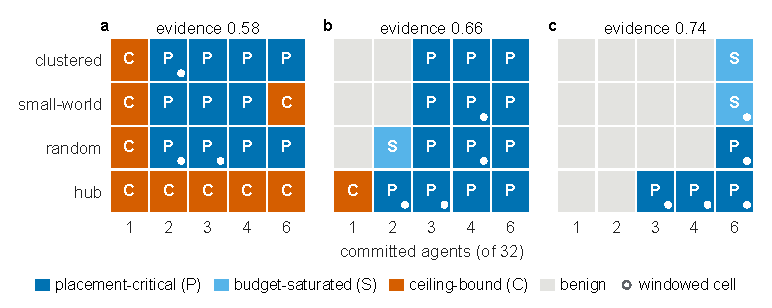
\includegraphics[width=\linewidth]{figures/fig_regime_map.pdf}
  \caption{Regime of each of the 60 cells of the belief-capture benchmark, at zero latency. Panels (a)--(c) show the three evidence strengths; within a panel, rows are topologies and columns are the number of committed agents. Each cell is colored by its regime. White dots mark the twelve windowed cells used for the placement-versus-budget comparison.}
  \label{fig:regime}
\end{figure}

\paragraph{Regimes}
We label each cell by preregistered rules applied in order. Let $p_{\text{base}}$ be the cell's capture rate with no checks, $p_{\text{ref}}$ the best prevention rate of the onset-informed reference over budgets, $p_{\text{uni}}^{B}$ the prevention rate of uniform placement with $B$ checks, and $p_1^{\star}$ the best prevention rate of any single-check policy. A cell is \textbf{benign} if $p_{\text{base}} < 0.10$; \textbf{ceiling-bound} if $p_{\text{ref}} \le 0.05$; \textbf{placement-critical} if $p_1^{\star} \ge 2\max(p_{\text{uni}}^{1}, 0.02)$ and $p_1^{\star} \ge 0.10$; \textbf{budget-saturated} if $\max_{B \in \{2,3\}} p_{\text{uni}}^{B} \ge p_{\text{ref}} - 0.05$; and intermediate otherwise. Figure~\ref{fig:regime} shows the result. Placement-critical cells are the largest group (28 of 60, 47\%), ceiling-bound cells form 17\% (10), and budget saturation is rare (3 cells, 5\%). We had preregistered that all three regimes would each cover at least 10\% of cells; budget saturation did not.

\paragraph{The window rule holds}
We simulated every schedule of one to three checks over rounds 2 to 15, $\binom{14}{1}+\binom{14}{2}+\binom{14}{3} = 469$ schedules, for each of the 3{,}000 cell--seed pairs. In every captured run, the rounds at which a single check prevents capture form an interval, and whether a schedule of two or three checks prevents capture is predicted by whether it meets that interval in all but 8 of 642{,}460 cases; the exceptions come from the benchmark detector removing an honest agent, which (A2) excludes. In each of the twelve windowed cells defined below, every window that exists opens at round 2, the first allowed check (Figure~\ref{fig:windows}a). One check at round 2 therefore attains the clairvoyant bound, and so does the best fixed schedule chosen on half of the seeds and scored on the other half, at every budget: its held-out prevention rate is 0.62 with one, two, or three checks. Across all 41 cells in which any capture is preventable, the best single round matches the bound in 38 and falls one run short in the other three.

\begin{figure}[!tbp]
  \centering
  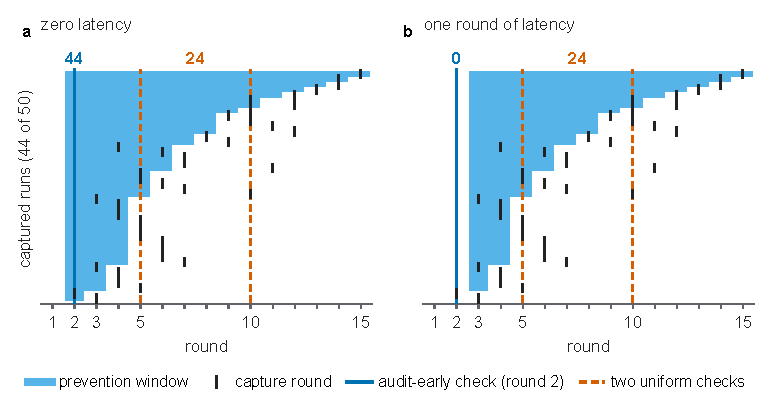
\includegraphics[width=\linewidth]{figures/fig_windows.pdf}
  \caption{Prevention windows of the 44 captured runs (of 50 seeds) in one windowed cell, with 4 committed agents, evidence 0.74 and a hub topology, at zero latency (a) and with one round of latency (b). Each row is one run: the bar spans the rounds at which a single check prevents capture, and the tick marks the capture round without checks. Rows are in the same order in both panels. The numbers above the lines count the runs prevented by the audit-early check at round 2 and by two uniform checks at rounds 5 and 10. Where a window ends after the capture round, removing the committed agents reverses a capture already counted (Section~\ref{sec:ceiling}). We show this cell because its windows end in the most distinct rounds; over all twelve windowed cells every window opens at round 2 at zero latency (374 runs) and at round 3 with one round of latency (256 runs).}
  \label{fig:windows}
\end{figure}

\paragraph{Where the first check lands decides the registered comparison}
The preregistered comparison runs on the \textbf{windowed cells}, those whose median capture round lies between 3 and 10, fixed before the comparison and blind to its outcome. Twelve cells qualify, eleven of them placement-critical and one budget-saturated. In each, we compare the best single-check policy against uniform placement with twice the budget. The single check prevents more captures in all 12 cells (mean gain $+0.39$, 95\% CI $[+0.26, +0.54]$, $p = 2.4\times10^{-4}$) and makes more timely catches in 11, with one tie (mean $+0.41$, CI $[+0.25, +0.58]$, $p = 4.9\times10^{-4}$). Against uniform placement with three times the budget, the second registered contrast, it wins in 12 of 12 cells on prevention (mean $+0.31$) and in 11 of 12 on timely catch, with one tie (mean $+0.30$). All four Holm-adjusted $p$-values are at most $9.8\times10^{-4}$. The best single-check policy is the same in every windowed cell, audit-early, whose single check falls at round 2. The window rule says what this contrast measures. Uniform placement checks first at round 5 or round 4, and many windows have closed by then; uniform spacing that starts at round 2, $\{2, 8\}$ or $\{2, 6, 11\}$, prevents exactly as many captures as the single check in all 12 cells. A larger budget does no harm once its first check lands in the window.

\paragraph{Robustness to the capture threshold}
The 80\% capture threshold decides when failure becomes irreversible, so we reran the sweep with thresholds of 60\%, 70\%, and 90\% under a protocol written before the run. The number of windowed cells changes with the threshold (7, 8, 12, and 16 at 60\% through 90\%), but the single check prevents more captures than two uniform checks in every windowed cell at every threshold except for one tie at 90\%, with mean gains between $+0.31$ and $+0.43$ (Table~\ref{tab:sens}). Placement-critical cells stay between 25 and 30 of 60.

\begin{table}[!tbp]
  \caption{Sensitivity of the regime map and of the placement-versus-budget comparison on the belief-capture benchmark. Upper block: detector varied at the registered 80\% capture threshold. Lower block: capture threshold varied with the benchmark detector at 0.50. Columns give the number of placement-critical (P), ceiling-bound (C), and budget-saturated (S) cells out of 60; the number of windowed cells; the number of windowed cells in which one check beats two uniform checks on prevention, with the mean gain; and the highest false-intervention rate on fault-free runs (detector rows only).}
  \label{tab:sens}
  \small
  \setlength{\tabcolsep}{4pt}
  \begin{tabular}{@{}lrrrrcr@{}}
    \toprule
    setting & P & C & S & windowed & prevention & false \\
     & & & & & wins, mean & intervention \\
    \midrule
    detector threshold 0.35 & 28 & 6 & 5 & 12 & 12/12, $+0.36$ & 1.00 \\
    detector threshold 0.40 & 27 & 7 & 5 & 12 & 12/12, $+0.36$ & 1.00 \\
    detector threshold 0.45 & 28 & 10 & 3 & 12 & 12/12, $+0.39$ & 0.36 \\
    detector threshold 0.50 (benchmark) & 28 & 10 & 3 & 12 & 12/12, $+0.39$ & 0.02 \\
    detector threshold 0.55--0.65 & 24 & 14 & 3 & 12 & 9/12, $+0.29$ & 0.00 \\
    perfect detector & 30 & 8 & 3 & 12 & 12/12, $+0.39$ & 0.00 \\
    \midrule
    capture threshold 60\% & 28 & 12 & 4 & 7 & 7/7, $+0.31$ & -- \\
    capture threshold 70\% & 30 & 10 & 2 & 8 & 8/8, $+0.34$ & -- \\
    capture threshold 80\% (registered) & 28 & 10 & 3 & 12 & 12/12, $+0.39$ & -- \\
    capture threshold 90\% & 25 & 12 & 0 & 16 & 15/16, $+0.43$ & -- \\
    \bottomrule
  \end{tabular}
\end{table}

\paragraph{Online triggers}
The suspicion-triggered policy never fired in any of the 3{,}000 committed runs, while it intervened in 2.7\% of fault-free runs. Its signal, a rise in the round's mean confidence, is as large when honest agents converge on the truth as when they are captured, so the threshold calibrated on fault-free runs is never reached first under capture. A passive signal that cannot tell convergence from capture cannot place a check.

\paragraph{When the window moves}
The window rule predicts that a fixed early check fails once windows stop opening at a known round. We tested two such cases, registered before the runs. A \textbf{schedule-aware adversary} makes its committed agents copy an honest agent's message in exactly the rounds a deterministic schedule reads; it cannot see the draw of a random schedule. At zero latency this cuts the prevention of the audit-early check by 0.44 on the windowed cells (CI $[-0.59, -0.31]$, 12 of 12). One random check does no better than the evaded fixed check (5 wins, 4 losses, 3 ties; we had predicted at least 9 wins), but three random checks beat it in 12 of 12 cells (mean $+0.15$, CI $[+0.11, +0.20]$), as randomized inspection would predict~\cite{blocki2015auditgames}. The adversary pays for its camouflage, because copying honest messages also stops it from pushing: among runs captured without checks in which the evaded check removes no one, 24\% are no longer captured. With one round of latency the camouflage falls in round 1 and this share rises to 87\%, so that arm measures the adversary's cost more than the schedules. A \textbf{delayed onset}, with committed agents behaving honestly until a round drawn from 1 to 8, mostly removes capture within 15 rounds instead of moving it: the capture rate on the windowed cells falls from 0.745 to 0.113, the remaining captures come from early onsets, and the round-2 check stays best (uniform with two checks loses to it in 10 of 12 cells, against our prediction). A longer horizon would be needed to test random onset on this benchmark; Section~\ref{sec:s2} tests it on a stream built for it.

\section{Latency Costs What the Detector's History Requirement Costs}
\label{sec:latency}

One round of reading delay sharply reduces what the benchmark detector can prevent. Replacing the detector shows that the cost comes from the detector needing two messages per agent: for detectors that need one, the same delay costs nothing.

\begin{figure}[!tbp]
  \centering
  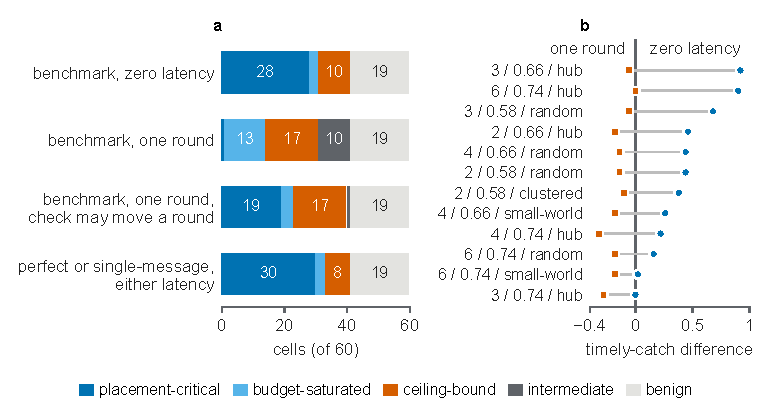
\includegraphics[width=\linewidth]{figures/fig_latency.pdf}
  \caption{Effect of one round of overseer latency. (a) Regime of the 60 cells for the benchmark detector at zero latency, at one round of latency with the fixed policy library, and at one round of latency when each policy may move its single check by one round, and for the perfect and single-message detectors, whose maps are identical at both latencies (Table~\ref{tab:latency}); segments of fewer than five cells are unlabeled. (b) Timely-catch difference between the best single check and uniform placement with two checks in each windowed cell (labeled committed agents / evidence strength / topology), at zero latency (circles) and at one round of latency with the fixed library (squares). Positive values favor the single check.}
  \label{fig:latency}
\end{figure}

\paragraph{The benchmark detector}
With one round of latency, the benchmark detector cannot flag anyone at round 2: every agent has sent exactly one message by then, so the detector's history-dependent behavioral term is zero, and the two remaining terms cannot both be nonzero, which caps the score at 0.4, below the 0.5 threshold. Enumeration confirms that a round-2 check with one round of latency is identical to no check in all 3{,}000 cell--seed pairs, and every window on the windowed cells now opens at round 3 (Figure~\ref{fig:windows}b). Audit-early and front-loaded schedules place their single check at round 2, so with a fixed library the regime map changes sharply (Figure~\ref{fig:latency}a): placement-critical cells fall from 28 to 1, budget-saturated cells rise from 3 to 13, ceiling-bound cells from 10 to 17, and ten former placement-critical cells become intermediate. On the windowed cells the single check now loses on timely catch in 11 of 12 (mean $-0.15$; Figure~\ref{fig:latency}b). Letting the check move by one round recovers the advantage: when each cell's check round is chosen on half of the seeds and scored on the other half, the chosen round is 2 in all twelve windowed cells at zero latency and 3 in all twelve at one round of latency, and the single check again beats two uniform checks on held-out seeds in 12 of 12 cells on prevention (mean $+0.20$, CI $[+0.13, +0.30]$, $p = 2.4\times10^{-4}$) and 11 of 12 on timely catch (mean $+0.26$, $p = 4.9\times10^{-4}$). What latency cannot recover is the prevention lost in the round it skips: over the 41 non-benign cells, the median clairvoyant bound halves from 0.24 to 0.12, and the median prevention of the onset-informed reference from 0.18 to 0.08.

\begin{table}[!tbp]
  \caption{Latency cost by detector on the belief-capture benchmark (registered protocol supplement). Regime counts out of 60 cells; clairvoyant bound as the mean prevention rate over the 12 windowed cells and the median over the 41 non-benign cells; false-intervention rate of a single check on fault-free runs, averaged over check rounds.}
  \label{tab:latency}
  \small
  \setlength{\tabcolsep}{4pt}
  \begin{tabular}{@{}llrrrrccc@{}}
    \toprule
    & & & & & & \multicolumn{2}{c}{clairvoyant bound} & false \\
    \cmidrule(lr){7-8}
    detector & latency & P & C & S & I & windowed & non-benign & intervention \\
    \midrule
    benchmark & zero & 28 & 10 & 3 & 0 & 0.62 & 0.24 & 0.010 \\
    benchmark & one round & 1 & 17 & 13 & 10 & 0.43 & 0.12 & 0.007 \\
    single-message & zero & 30 & 8 & 3 & 0 & 0.62 & 0.24 & 0.000 \\
    single-message & one round & 30 & 8 & 3 & 0 & 0.62 & 0.24 & 0.000 \\
    perfect & zero & 30 & 8 & 3 & 0 & 0.62 & 0.24 & 0.000 \\
    perfect & one round & 30 & 8 & 3 & 0 & 0.62 & 0.24 & 0.000 \\
    \bottomrule
  \end{tabular}
\end{table}

\paragraph{Detectors that need one message}
We reran the sweep with two other detectors, keeping cells, seeds, and schedules fixed. The \textbf{perfect detector} flags every committed agent that has sent at least one message in the visible prefix and never flags an honest agent. The \textbf{single-message detector} applies the benchmark's confidence term to the mean confidence of an agent's visible messages, $\min(1, \max(0, (\bar c - 0.9)/0.09))$, with its threshold set on fault-free runs only, before any committed cell ran, to the lowest value whose false-intervention rate is at most 0.02, the benchmark detector's rate in Table~\ref{tab:sens} (0.72 at zero latency, 0.70 at one round). For both, one round of latency changes nothing (Table~\ref{tab:latency}): the regime counts, the clairvoyant bound, and the reference's prevention are identical at both latencies. A check at round 2 that reads only round 1 already sees one message from every committed agent, and removal still acts before round 2's update, so the window opens at round 2 either way, as Proposition~\ref{prop:window} predicts for $k = 1$. The single-message detector matches the perfect one here because committed agents announce confidence 0.99 from their first message while honest agents start near their private evidence. That signal is easy to remove: the jitter adversary of Section~\ref{sec:hindsight} adds noise to exactly this confidence, and on LLM panels it erases timely detection. The general point stands without the particular detector: the cost of a round of delay is set by how many rounds of an agent's history the detector must see.

\section{No Window Exists When Capture Is Immediate or Rare}
\label{sec:ceiling}

In about a sixth of the benchmark no checking schedule prevents more than 5\% of runs from failing. Two mechanisms account for all ten such cells: capture before the first allowed check, and capture too rare for the absolute prevention rule to be met. A perfect detector moves only two of them out of this regime.

\paragraph{The exact bound and the deadline}
Across the ten ceiling-bound cells, the clairvoyant bound prevents 13 of 326 captures (4.0\%), consistent with the registered limit of 5\% prevention. Labels assigned with the onset-informed reference agree with the exhaustive bound in 57 of 60 cells. The capture round approximates the end of the window but does not equal it. With the perfect detector at zero latency, the last round at which a single check prevents capture equals the capture round in the median run, falls at least one round earlier in 45\% of captured runs, and lies after the capture round in 125 of 1{,}412, where removing the committed agents reverses a capture already counted. This is why checking at the capture round makes 98.5\% of the achievable timely catches but only 50\% of the achievable preventions.

\paragraph{Capture before the first allowed check}
Six ceiling-bound cells, five on hub graphs and one on a small-world graph, all with weak evidence, are captured in round 1 or 2 in nearly every run; five of them have a median capture round of 1. Their windows close before round 2, the first check we allow, because the benchmark detector cannot flag anyone from a single message. Allowing a check within round 1 at zero latency, the perfect detector prevents 246 of the 249 captures in the five round-1 cells and all 48 in the sixth. These cells are ceiling-bound because no check is allowed before the first belief update, a property of the oversight protocol and of the detector's history requirement, not of how good the detector is.

\paragraph{Rare capture}
The other four ceiling-bound cells are captured in only 10--24\% of runs. In relative terms the bound is not low there: it prevents 11 of their 29 captures (38\%), and the perfect detector 22 (76\%). They are ceiling-bound because the registered rule measures prevention in absolute terms, and a cell that rarely fails cannot gain 5 points. Under the perfect detector, still checking from round 2, two ceiling-bound cells become placement-critical, one of these rare-capture cells and the early cell whose median capture round is 2.5, which is why its placement-critical region grows from 28 to 30 cells; the placement-versus-budget comparison is unchanged under it (Table~\ref{tab:sens}).

\paragraph{Detector threshold}
Near the benchmark value, the detector's threshold leaves the regime map unchanged. Thresholds of 0.45 and 0.50 produce identical regime counts and comparisons, although the false-intervention rate on fault-free runs is 0.36 at 0.45 against 0.02 at 0.50. Lower thresholds appear to shrink the ceiling (to six cells at 0.35), but they flag an honest agent in every fault-free run. Higher thresholds (0.55--0.65) miss more committed agents, the ceiling grows to 14 cells, and the single check wins in 9 of 12 windowed cells on prevention.

\section{Early Schedules Do Not Transfer to Faults with Random Onset}
\label{sec:s2}

On the capture benchmark every fault starts at round 1, so every window opens at the same round and an early check wins. When onset is random the window opens at the onset, and a schedule must cover where onsets fall. We test this on a stream built for it, which differs from the capture benchmark in three ways at once: one reasoner instead of a group, a delay penalty instead of a sharp deadline, and random onset. It tests whether the placement rule transfers, not whether the regime map does.

\begin{figure}[!tbp]
  \centering
  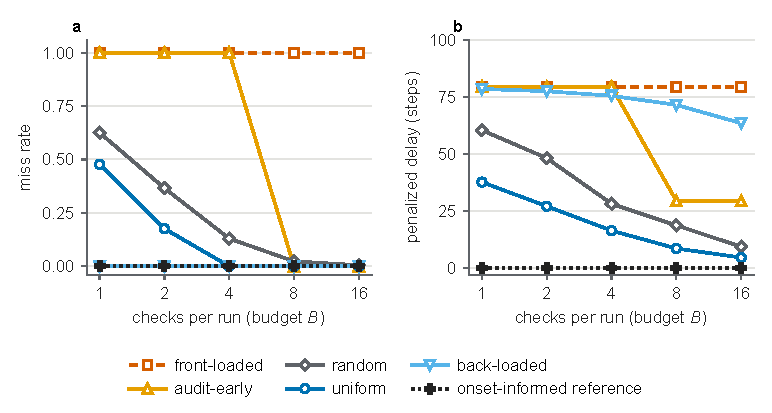
\includegraphics[width=\linewidth]{figures/fig_s2_missrate.pdf}
  \caption{Rule-shift stream with onset drawn uniformly from steps 40--120 of 160, pooled over the nine cells whose candidate set contains the target rule and whose rules disagree on some inputs. (a) Fraction of runs in which the shift is never detected; front-loaded and audit-early coincide at 1.0 for budgets up to four, and back-loaded coincides with the reference at 0. (b) Penalized delay: steps from onset to detection, with undetected shifts charged the remaining horizon.}
  \label{fig:s2}
\end{figure}

Figure~\ref{fig:s2} shows the results on the nine cells whose candidate set contains the target rule and whose two rules can be told apart. Audit-early placement misses every shift at budgets of 1, 2, and 4, because geometric spacing puts all its checks at steps 2--16, before the earliest possible onset; front-loaded placement fails the same way. Uniform placement degrades gradually, with miss rates of 0.48, 0.18, and 0.00 at those budgets, and the onset-informed reference, which checks at the true onset, never misses. Penalized delay shows a second failure that miss rate hides: back-loaded placement rarely misses but detects near the end of the stream, and audit-early, once it stops missing at eight checks, still detects late. We had preregistered that audit-early's advantage would carry over to this stream; it did not in any of the three registered high-separability cells.

Audit-early fails under other onset distributions too. In a separate sweep with 50 new seeds on the same nine cells, onset drawn from steps 2--30, where early checking should have the advantage, still leaves audit-early missing 0.97, 0.87, and 0.46 of shifts at budgets of 1, 2, and 4, while uniform placement misses none: geometric spacing puts the checks at steps 2, 4, 8, and 16, so a shift after the last check goes unseen. A wider onset range (steps 5--155) or a bimodal distribution leaves audit-early at 1.00, 1.00, and 0.91, and 1.00, 1.00, and 0.64. In window terms, uniform spacing covers windows spread over the stream and geometric spacing covers only its start.

An onset estimate helps only when it is accurate. When we add noise to the onset given to a single-check placement policy, onset-guided placement stops beating uniform placement once the estimation error reaches 8.2 steps (95\% CI $[3.0, 19.1]$, over 24 seeds), about a tenth of the 80-step range over which onset varies. When the candidate set excludes the target rule, nothing can be detected: in all ten such cells at budgets up to four, every policy, including the reference, misses every shift, because the window is empty for this detector.

\section{Hindsight Accuracy Overstates Decision-Time Detection}
\label{sec:hindsight}

A monitor's accuracy on completed transcripts is a poor guide to what it can detect before the deadline, and choosing monitors by it selects signals that need history the deadline does not provide.

\begin{figure}[!tbp]
  \centering
  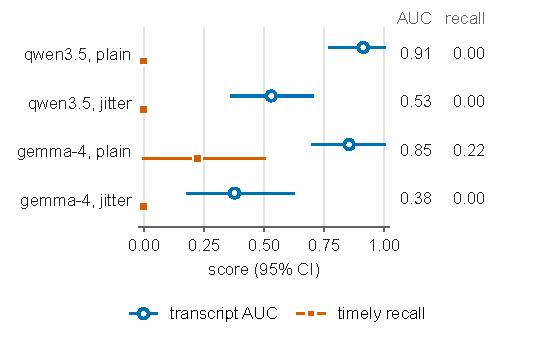
\includegraphics[width=0.72\linewidth]{figures/fig_dissociation.pdf}
  \caption{Hindsight and decision-time detection on two current model families. For each family and adversary (plain or jitter), the benchmark detector's AUC on completed transcripts (circles) and its timely recall at the last round at which removal could prevent capture, with one round of latency (squares). Lines are 95\% bootstrap intervals over panels; the values are listed on the right.}
  \label{fig:dissoc}
\end{figure}

\paragraph{Two current model families}
Capture replicates on both families: all 20 qwen3.5 panels and all 20 gemma-4 panels are captured. Figure~\ref{fig:dissoc} shows the benchmark detector at its deployed threshold of 0.5. Under the plain adversary, the detector reaches a transcript AUC of 0.91 on qwen3.5 (95\% CI $[0.77, 1.00]$, resampling panels), yet its timely recall at the deadline is 0.00 with one round of latency, in every bootstrap replicate. On gemma-4 the transcript AUC is 0.85 $[0.70, 1.00]$ and timely recall 0.22 $[0.00, 0.50]$. The round-by-round record shows why. At round-2 captures, the most common case on gemma-4, the detector's AUC at the deadline is 0.38, below chance, and it rises to 0.99 one round later, after capture is decided. With zero latency, timely recall rises to 0.85 on gemma-4 and 0.30 on qwen3.5. The jitter adversary lowers transcript AUC to 0.53 on qwen3.5 and 0.38 on gemma-4 and leaves timely recall at 0.00 at either latency. This is the mechanism of Section~\ref{sec:latency} on real models: the detector needs a second message, a round-2 capture read one round late leaves one, and the window closes before the detector can act. We had preregistered timely recall of zero for both families; gemma-4's 0.22 instead shows that slower captures leave a little room. With 20 trials per family, these intervals are wide, and the comparison between families is qualitative.

\paragraph{Thirteen monitors}
We then replay thirteen monitors over all 130 panels. The benchmark detector combines three terms computed on the visible prefix: a provenance term $s_1$ (how many agents send the same self-supporting message this round), a behavioral term $s_2$ (the product of an agent's confidence constancy, claim constancy, and confidence level, undefined before two messages exist), and a divergence term $s_3$ (how often an agent cites evidence against its own claim), weighted $0.4$, $0.4$, and $0.2$. The archived logs record whether a message cites evidence but not which way it points, so $s_3$ cannot be replayed, and the replayed benchmark detector is $0.4\,s_1 + 0.4\,s_2$. It therefore orders agents exactly as the equal-weight variant $0.5\,s_1 + 0.5\,s_2$ does, which is why the two rows of Table~\ref{tab:zoo} are identical. The other monitors are $s_1$ and $s_2$ alone, three reweightings of them, a raw signature-reuse count, and six single signals: mean confidence, confidence constancy, claim constancy, high-confidence share, round-1 confidence, and evidence rate. The unit is one agent in one trial, labeled committed or honest, so timely recall is the share of committed agents flagged by the deadline, taken as the capture round. On the capture benchmark the last preventing round falls before the capture round in 45\% of runs (Section~\ref{sec:ceiling}), so this deadline is generous to the monitors. Each monitor's threshold is set so that it flags 6.25\% of honest agents on completed transcripts, the benchmark's deployed rate; several monitors take only a few distinct values, so honest agents tied at the threshold are flagged with the probability that makes the rate exactly 6.25\%. With one round of latency, 862 of the 948 agent--trial units remain scoreable at the deadline: six trials are never captured, and four are captured in round 1, leaving no prefix to read.

\begin{figure}[!tbp]
  \centering
  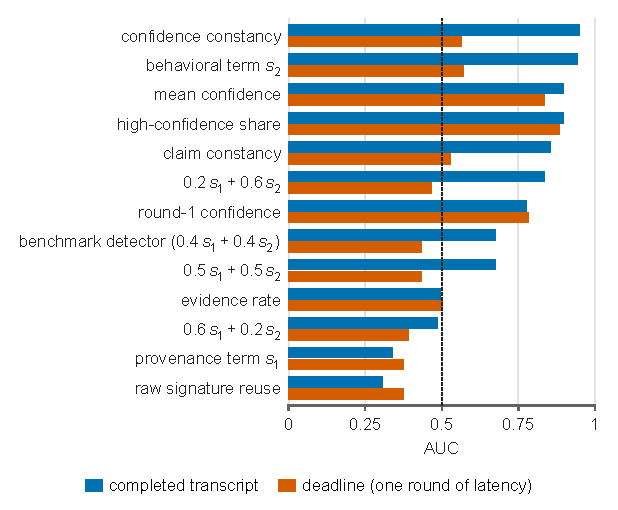
\includegraphics[width=0.8\linewidth]{figures/fig_zoo.pdf}
  \caption{AUC of each of the thirteen monitors on completed transcripts (upper bar) and at the last timely round with one round of latency (lower bar), over all 130 panels, in the order of Table~\ref{tab:zoo}. The dashed line marks chance (AUC 0.5).}
  \label{fig:zoo}
\end{figure}

The main effect is a drop in level for the monitors that need history (Figure~\ref{fig:zoo}, Table~\ref{tab:zoo}). The best monitor on transcripts, confidence constancy, falls from 0.95 AUC to 0.56 at the deadline. The monitors that read a single round keep most of their accuracy: high-confidence share falls only from 0.90 to 0.88 and reaches the highest timely recall, 0.36 (CI $[0.29, 0.47]$). Selecting the monitor by transcript AUC would therefore pick a constancy signal that is nearly uninformative when a check could still help, while selecting by deadline AUC would pick one that works. Even the best monitor recalls about a third of the committed agents in time. Setting each threshold on deadline data instead lowers the best recall to 0.27. Raising the false-positive rate narrows the gap only at a high price: the best timely recall is 0.12 at a 2\% rate, 0.29 at 5\%, and 0.67 at 10\%, which means flagging one honest agent in ten.

Rankings change less than levels. Restricting both sides to the units that are scoreable at the deadline, the rank agreement between transcript AUC and deadline AUC is Kendall $\tau = 0.64$ with one round of latency and 0.97 with zero latency, and between transcript and deadline recall at equal false-positive rates it is 0.72 and 0.90. The preregistered comparison, transcript AUC against deadline recall computed with the registered threshold rule, gives $\tau = 0.51$ $[0.36, 0.56]$, which passes the registered criterion ($\tau \le 0.6$). However, comparing transcript AUC with transcript recall, without changing the time of evaluation, already gives $\tau = 0.46$, so most of that reordering comes from switching between AUC and recall rather than from timing. Timing changes which monitors can be computed at all. Constancy signals need at least two rounds of history; with one round of latency, a round-2 capture leaves one round visible, and confidence constancy recovers only 0.12 recall. With zero latency it is computable and leads all monitors at 0.63.

\begin{table}[!tbp]
  \caption{The thirteen monitors over all 130 panels: AUC on completed transcripts, AUC at the last timely round, and timely recall when 6.25\% of honest agents are flagged on completed transcripts, with ties at the threshold broken at random. Deadline values use one round of latency (948 transcript units, 862 units scoreable at the deadline).}
  \label{tab:zoo}
  \small
  \begin{tabular}{lccc}
    \toprule
    monitor & transcript AUC & deadline AUC & timely recall \\
    \midrule
    confidence constancy & 0.95 & 0.56 & 0.12 \\
    behavioral term $s_2$ & 0.94 & 0.57 & 0.10 \\
    mean confidence & 0.90 & 0.83 & 0.24 \\
    high-confidence share & 0.90 & 0.88 & 0.36 \\
    claim constancy & 0.86 & 0.53 & 0.22 \\
    $0.2\,s_1 + 0.6\,s_2$ & 0.83 & 0.47 & 0.05 \\
    round-1 confidence & 0.78 & 0.78 & 0.00 \\
    benchmark detector ($0.4\,s_1 + 0.4\,s_2$) & 0.68 & 0.43 & 0.01 \\
    $0.5\,s_1 + 0.5\,s_2$ & 0.68 & 0.43 & 0.01 \\
    evidence rate & 0.50 & 0.50 & 0.06 \\
    $0.6\,s_1 + 0.2\,s_2$ & 0.49 & 0.39 & 0.01 \\
    provenance term $s_1$ & 0.34 & 0.38 & 0.00 \\
    raw signature reuse & 0.31 & 0.38 & 0.00 \\
    \bottomrule
  \end{tabular}
\end{table}

\section{Discussion}
\label{sec:discussion}

\paragraph{What an oversight tool should estimate}
The window rule turns schedule design into three estimates. The first is when the window opens: the earliest round at which the detector, read at the deployment's latency, can identify the fault. It depends on the detector's history requirement and on the overseer's delay together, which is why one round of delay halved the benchmark detector's median clairvoyant bound and cost a single-message detector nothing (Section~\ref{sec:latency}). The second is when it closes, approximated by the moment failure becomes irreversible but often a round earlier (Section~\ref{sec:ceiling}). The third is how much windows vary across runs. When they share a round, as when faults start at once, one check at that round is the whole schedule and extra budget buys nothing (Section~\ref{sec:s1}). When they move, because onset is random (Section~\ref{sec:s2}) or because an adversary avoids known checks (Section~\ref{sec:s1}), checks must be spread or randomized to cover them, and choosing $B$ checks becomes a covering problem over the distribution of windows. Monitors should be compared by their recall at the window's end, at the deployment's own latency, rather than by transcript AUC (Section~\ref{sec:hindsight}).

\paragraph{Using the results without the benchmark's parameters}
A deployment does not observe minority size or evidence strength, the parameters that define our cells. It can observe its own latency, how much history its detector needs, the timing of past incidents, and how quickly failures became irreversible in them. Without an onset estimate accurate to about a tenth of the onset range, uniform spacing is the safer default: on the rule-shift stream it degraded gradually (miss rates 0.48, 0.18, 0.00 at one, two, and four checks) while the early schedules missed every shift. Where failures complete before the first possible check, more checks during the run add nothing; what helps is an earlier intervention point or a detector that works from the first message.

\paragraph{Limitations}
The bounds are clairvoyant bounds on fixed detectors. They limit what checking schedules can achieve; they do not measure people. Checks have unit cost, whereas a real overseer's reading cost grows with the length and complexity of what is read, and intervention here is automatic removal rather than a human decision. Proposition~\ref{prop:window} assumes that a check flags all faulty agents or none and no honest one; detectors with partial or noisy detection make windows fuzzy, and the rule then holds only approximately, as the 8 exceptions on the benchmark show. The two substrates are controlled model systems chosen because their fault dynamics can be varied, the deadline is sharp in one and gradual in the other, and the LLM panels are small. The committed LLM agents are prompted to argue for the false claim, and the confidence signals that survive to the deadline may reflect that prompt; the jitter adversary removes them. Our two strategic tests are narrow: the evading adversary gives up pushing whenever it hides, and delayed onset within 15 rounds mostly prevents capture rather than moving it, so stronger adversaries and longer horizons remain to be tested. The regime rules' own thresholds were fixed by preregistration and not varied. Domains with partly reversible failures, overlapping faults, or longer horizons may shift the regime boundaries, and the released replay tooling can express these variations. The most important open question is whether operators who are shown these quantities, including an explicit statement that no check can help in a setting, allocate their attention better or disengage~\cite{parasuraman1997,lee2004trust}; answering it requires a study with people. The substrates and archived panel logs are shared with other work that uses the same testbeds; all results reported here were computed for this paper.

\section{Conclusion}

We modeled oversight checks as reads of a causal prefix under a budget, and showed that when flagged agents are removed for good, a schedule prevents a failure exactly when one of its checks lands in the run's prevention window. On a benchmark where every schedule could be enumerated, the rule held in all but 8 of 642{,}460 multi-check outcomes. Its consequences held as well: one check at the window's opening matched the clairvoyant bound, extra checks mattered only when windows moved, one round of delay cost what the detector's need for history cost, and the settings no schedule helped were captured before the first allowed check or rarely captured at all. On LLM panels, the most accurate monitors on completed transcripts relied on history that the deadline does not provide. Oversight tools should therefore estimate when their detector can first identify a fault, when intervention stops helping, and how much these moments vary, and should report recall at the deadline. The next step is to test whether people overseeing agents use these quantities well.

\backmatter

\section*{Statements and Declarations}

\bmhead{Funding} No funding was received for conducting this study.

\bmhead{Competing interests} The author has no competing interests to declare that are relevant to the content of this article.

\bmhead{Ethics approval and consent to participate} Not applicable. The study involves no human participants and no personal data; all agents are simulated programs or language models.

\bmhead{Data availability} The simulation outputs, LLM-panel transcripts, and the preregistered protocols are available at \url{https://github.com/xxx12e/decision-time-oversight}.

\bmhead{Code availability} The simulation, replay, and analysis code, including the script that checks every reported number against the result files, is available at \url{https://github.com/xxx12e/decision-time-oversight}.

\bmhead{Author contribution} H.L. designed the study, implemented and ran the experiments, analysed the results, and wrote the manuscript.

\bibliography{references}

\end{document}
